\section{Assuring Safe Perception}\label{sec:proofrule}
%Willem and Martin\\
%4,5 pages	concluded at page 13\\

In this section we focus on bounding the impact of misperception through incorrect classifications. Together with the quality guarantees provided by sensor fusion, this allows to bound the risks of misperception for beliefs of the ego vehicle, as long as sensor completeness is guaranteed, and the distribution of real traffic matches the distributions used in the training phase of the learning components. 

\subsection{Classifier Analysis}
An ontology $\mathcal O=(\mathcal L,\sqcap,\sqcup)$ is a complete distributive lattice over a set $\mathcal L$ of labels representing object class identifiers. The unique complement of $l\in\mathcal L$ is denoted by $\overline l$. The induced non-strict partial order on $\mathcal O$ is denoted by $\sqsubseteq$ and its strict variant by $\sqsubset$. We say that a label $l\in\mathcal L$ is more specific (or, vice versa, broader) than a label $l'\in\mathcal L$ if $l\sqsubset l'$ ($l'\sqsubset l$, respectively). A classifier $c_l$ ---usually obtained by training a machine-learning framework--- for the label $l\in\mathcal L$ takes an artifact $a$ as input and returns a numerical value $c_l(a) \in [\min,\max]$ which corresponds to its degree of conviction that the artifact $a$ is of type $l$.
Given an upper threshold $g_l^+$ and a lower threshold $g_l^-$ with $g_l^+\geq g_l^-$, we define the label assignment for an artifact $a$ as follows
\begin{gather*}
    \Label(c_l,g_l^+,g_l^-)(a) = \left\{
    \begin{array}{ll}
    l & \text{ if } c_l(a) \geq g_l^+\\
    \overline l & \text{ if } c_l(a) < g_l^-\\
    \top & \text{ otherwise.}
    \end{array}\right.
\end{gather*}
We use the short notation $\Label(c_l)(a)$ when the thresholds are fixed. 

There are various quality measures for classifiers. A classifier is usually evaluated against a given test data set $T$, where $T$ is correctly and completely labeled against a representative set of artifacts. Hence, for each label $l\in\mathcal L$, we obtain a partitioning of $T=T(l) \cup T(\overline l)$ into the set $T(l)$ of artifacts which are labeled with $l$ and its complement $T(\overline l)$. The corresponding numbers of elements in $T$ are denoted by $n_l$ and $n_{\overline l}$, respectively.

To analyze a classifier $c_l$ we are mainly interested in the relation between the threshold $g_l^+$, the true positive rate (\TPR), and the false positive rate (\FPR) on the one hand, and the relation between the threshold $g_l^-$, 
the true negative rate (\TNR), and the false negative rate (\FNR) on the other.
For each classifier we obtain two ROC curves (receiver operating characteristics):
\begin{itemize}
\item ROC curve $RP$ represents the relationship of $\TPR(g_l^+)$ and $\FPR(g_l^+)$,
where
\begin{gather*}
    \TPR(g_l^+) = \frac{ | T(l) \cap \{a |c_l(a) \geq g_l^+ \}|}{|T(l)|},\quad
    \FPR(g_l^+) = \frac{ | T(\overline l) \cap \{a| c_l(a) \geq g_l^+ \}|}{|T(\overline l)|}
\end{gather*}
\item ROC curve $RN$ represents the relationship of $\TNR(g_l^-)$ and $\FNR(g_l^-)$, where
\begin{gather*}
    \TNR(g_l^-) = \frac{ | T(\overline l) \cap \{a|c_l(a) < g_l^- \}|}{|T(\overline l)|},\quad
    \FNR(g_l^-) = \frac{ | T(l) \cap \{a|c_l(a) < g_l^- \}|}{|T(l)|}.
\end{gather*}
\end{itemize}

%Achtung! Hier kann es bei geänderten Umbrüchen zu Problemen kommen
\begin{wrapfigure}[16]{R}{0.44\textwidth}
    \vspace{-3em}
    \centering
    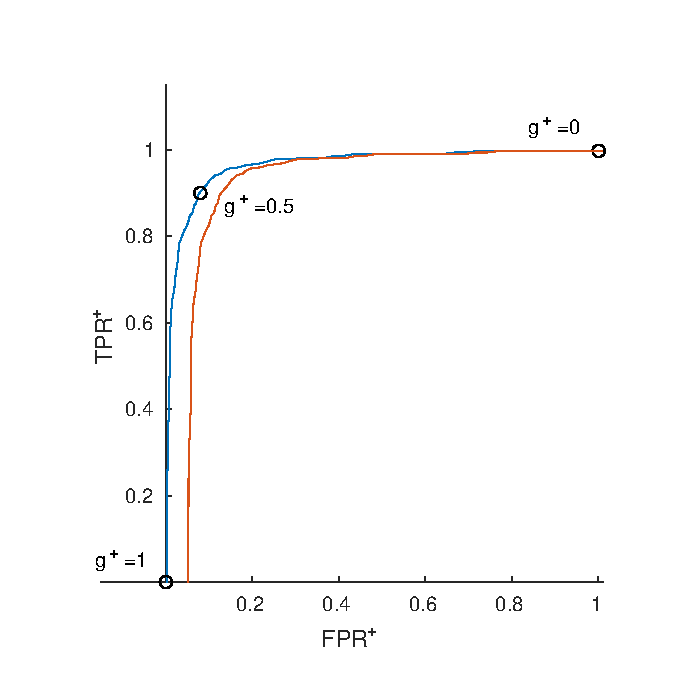
\includegraphics[width=0.44\textwidth]{ros}
    \caption{The ROS curve obtained by test data is in blue, the $\epsilon$-margin for a $\beta$ confidence is in red.}
    \label{fig:ros}
\end{wrapfigure}
The rates as given above are measured against the test data set $T$, which is independent from the training data set used for establishing the classifiers $c_l$. 

As the test data set $T$ constitutes a finite sample of the actual possible situations, the empirical rates TPR, FPR, TNR, and FNR are approximate only. According to Hoeffding's inequality we can, however, derive the following bounds for the actual false positive rates $\widehat\FPR$ and the actual false negative rate $\widehat\FNR$:
\begin{gather*}
    \FPR(g_l^+) + \epsilon \geq \widehat\FPR(g_l^+) 
    \text{ with confidence $\beta$ if } \beta \leq 1 - e^{-2|T(\overline l)|\epsilon^2}\text,\\
    \FNR(g_l^-) + \epsilon \geq \widehat\FNR(g_l^-)
    \text{ with confidence $\beta$ if } \beta \leq 1 - e^{-2|T(l)|\epsilon^2}\text.
\end{gather*}
The situation is depicted in Fig. \ref{fig:ros}. Note, that the rates above correspond to unknown conditional probabilities. E.g.\
$\widehat\FPR(g_l^+)$ represents the expected value of the conditional probability $P( c_l(a)\geq g_l^+ | a\in T(l))$.

\subsection{Classifier Optimization}
Let $\Phi$ be a formula that guards a safety-critical maneuver in the sense that the driving function will only adopt the maneuver when it has positive evidence of the validity of $\Phi$ in the current situation, implying that the maneuver would be avoided (and a safer substitute adopted) whenever $\Phi$ is violated \emph{or} evaluation of $\Phi$ remains inconclusive. 
Such formulae $\Phi$ are generated by the prediction component on the fly, reflecting massive Boolean combinations of conditions on individual cells of the occupancy grid, where both the particular cells referenced and the individual conditions vary situationally, i.e.\ the universe of such queries $\Phi$ is far too large to compute optimized detectors in advance.
E.g. $\Phi$ may safeguard a fast transit of a critical passage by ensuring that there are no humans on the sidewalk, where the geometric position of the sidewalk will depend on street geometry and position of the car in the lane, while the lookahead and thus number and distance of the cells depends on current speed, road conditions, etc. In such a setting $\Phi = \lit_1 \land \lit_2 \land \dots \land \lit_n$ is a conjunction of literals $\lit_i=\lnot A_i$ of the form ``it is false that there is a human at cell $c_i$''. The truth value of each atom $A_i$ directly depends on a classifier output, which is, in our example, a classifier for object class ``human''. Our goal is to find an optimal combination of threshold values for the related classifiers, separately for each cell,
such that the risk of misperception, i.e.\ the false-positive rate for evaluation of $\Phi$, is restricted to a given safety bound
$\epsilon$ while the availability, i.e.\ the true-positive rate for evaluation of $\Phi$, is maximized. In the following we show that
this problem can be translated into a polynomial optimization problem.

% To ease the argumentation, we stipulate that $\Phi$ being true increases
% the availability while $\Phi$ being false leads to safe
% maneuvers only. 
From an application perspective, the optimization problem at hand is to maximize the (actual) true positive rate of a formula $\Phi$ while ensuring that the (actual) false positive rate of $\Phi$ is below a given threshold $\epsilon$. Without loss of generality we assume that $\Phi$ is given in distributive normal form. We show how
to rewrite the initial optimization problem
\begin{align*}
  \textrm{maximize} &\ \TPR_\Phi&
  \textrm{s.t.} &\ \FPR_\phi\leq \epsilon\text.
\end{align*}

\begin{enumerate}
\item Let $\Phi = \phi_1 \lor \phi_2 \lor \phi_n$ be a disjunction of
  subformulas $\phi_1$, \dots, $\phi_n$. For any pair $\phi_i$ and $\phi_j$ with $i\neq j$ we assume that the formulas refer to disjoint regions in the occupancy grid. 
  $\Phi$ yields a false positive as soon as some $\phi_i$ does so \emph{and} no $\phi_j$ is truly positive at the same time. Consequently $\sum_{i=1}^n \FPR_{\phi_i} \geq \FPR_{\Phi}$. Due to the inequation $P(\phi \lor \psi) \leq P(\phi) + P(\psi)$ and
  the spatial separation of the formulas it holds that $\sum_{i=1}^n\TPR_{\phi_i} + \sum_{i \neq j}^n \FPR_{\phi_i}(1-\TPR_{\phi_j})\geq \TPR_\phi$,
  since the disjunction $\Phi$ is truely positive if and only if either at least one of the $\phi_i$ is, or there exist indices $i\neq j$ such that $\phi_i$ is falsely positive -- rendering $\Phi$ to be positive -- and $\phi_j$ is true, but not positive -- rendering $\Phi$ to be true.
  %\todo{MF: Ich fuerchte, dass können wir ohne einen geeigneten Prior ueber die situativ erwartete Haeufigkeit von $\Phi$ nicht vorteilhaft aufloesen. Denn hier muessen wir zwie bedingte Wahrscheinlichkeiten verknuepfen, die uber komplementaere Bedingungen reden.}
  %\todo{MF: Diese Abschaetzung gilt, ist aber nicht sehr nuetzlich, da sie die Maskierung eines FPs durch eine anderes TP vernachlaessigt und mithin zu viel zu hohen FPRs kommt.}
  Hence we restate the initial optimization problem as follows:
  \begin{align}
    \textrm{maximize} &\ \sum_{i} \TPR_{\phi_i}+\sum_{i\neq j}
    \FPR_{\phi_i}(1-\TPR_{\phi_j})& 
    \textrm{s.t.} &\ \sum_{i} \FPR_{\phi_i} \leq \epsilon\text.
    \label{eq:optimization2}
  \end{align}
  Any optimal solution of this optimization problem is also a
  feasible solution of the initial optimization problem, but not necessarily
  an optimal solution.
\item Let $\Phi = \lit_1 \land \lit_2 \land \dots \land \lit_n$
  be a conjunction of literals.
  %We want to ensure that the false negative
  %rate of $\Phi$ is below a given threshold $\epsilon$. Clearly,
  %$\Phi$ is false if at least one literal is a false positive.
  %On the other hand, $\Phi$ is positive if and only if all literals
  %are positive. Taking both arguments together yields that
  %$\Phi$ is a false positive if and only if all literals are false positives.

%  Recall that the rates under consideration correspond
%  to the expected values of conditional probabilities.
%  For stochastically independent events we have the identity 
%  $p(A_1|B_1)\cdot p(A_2|B_2) = p(A_1,A_2|B_1,B_2)$. Under the assumption that
%  the underlying classifiers of two literals are stochastically independent,
%  this allows us to represent the false negative rate of a conjunction as the
%  product of the literals. The same argument holds for the true positive rate.
  In duality to the argument for disjunctions we obtain that a conjunction $\Phi$ yields a true positive iff all its conjunctions $\phi_i$ do yield a true positive and that $\Phi$ yields a false negative iff at least one $\phi_i$ does and all the others yield some positive. Assuming stochastic independence %\todo{MF:Eine starke Annahme! Wie rechtfertigen?} 
  we obtain 
  $\TPR_\Phi = \prod_{i=1}^n \TPR_{\lit_i}$ and
  $\FPR_\Phi \leq \prod_{i=1}^n \FPR_{\lit_i}$.
  %
  %Hence, we are allowed to distribute a given threshold $\epsilon$ for the
  %false negative rate of $\Phi$, i.e.,
  %$\FPR_\Phi+\epsilon\geq\widehat{\FPR_\Phi}$ to the literals
  %$\prod\epsilon_i = \epsilon$ such that $\epsilon_i$
  %is an individual threshold for the false positive rate for the
  %literals $l_i$.
  Substituting the resulting polynomials into the optimization problem \eqref{eq:optimization2} yields a polynomial optimization problem over true positive and false positive rates of literals.
  %\begin{align*}
  %  \textrm{maximize} &\ \sum_i \prod_k \TPR_{\lit_{i,k}} + \sum_{i\neq j}\left(\prod_k\FPR_{\lit_{i,k}}\left(1-\prod_k\TPR_{\lit_{j,k}}\right)\right)\\ \textrm{s.t.} &\ \sum_i\prod_k \FPR_{\lit_{i,k}} \leq \epsilon\text.
  %\end{align*}
  %\begin{align*}
  %  \textrm{maximize} &\ \sum_i \prod_j \TPR_{\lit_{i,j}}& \textrm{s.t.} &\ \sum_i\prod_j \FPR_{\lit_{i,j}} \leq \epsilon\text.
  %\end{align*}
\item Let $\Phi$ be a single literal of the form $A$,
  where $A$ corresponds to the classifier $c_l$. Then the true-positive and false-negative rates of $c_l$ correspond to the corrected empirical rates $\widehat\TPR$ and $\widehat\FNR$, which are coupled to the thresholds $g_l^+$ and $g_l^-$ via the ROC curves. As a conservative polynomial approximation of these ROC curves can be substituted into the above optimization problem, we obtain constraints on the thresholds $g_l^+$ and $g_l^-$. 
\item Let $\Phi$ be a single literal of the form $\lnot A$,
  where $A$ corresponds to the classifier $c_l$.
  The false negative rate $\FNR_\Phi$ corresponds to the false positive rate
  of $c_l$, and likewise the true positive rate $\TPR_\Phi$ corresponds to the true negative rate of $c_l$. Again these are linked to the thresholds $g_l^+$ and $g_l^-$ via the corresponding ROC curves (corrected for the empirical error).  %E.g.\ let $\Phi$ be formula which guards a cell which we would
  %like to enter, where $\Phi$ is true if the cell is free of obstacles.
  % We have to ensure that the false positive rate of the
  % classifier $c_l$ is under a certain threshold, yielding a lower bound for
  % $g_l^+$. To optimize the true positive rate of $\Phi$, we optimize
  % the true negative rate of $c_l$, that is we aim for minimizing $g_l+$ with
  % $g_l^+\geq g_l^-$.
  
  % Clearly, for $\Phi=A$, where $A$ is an atom $A$ corresponding
  % to the classifier $c_l$, the false negative rate and true positive rate
  % of $\Phi$ coincides with the corresponding rates of $c_l$.
\end{enumerate}
Solving the resulting polynomial optimization problem on the individual thresholds of the classifiers will yield a classifier for the compound goal $\Phi$ which satisfies the desired bounds on its FPR, i.e.\ the likelihood of erratic adoption of risky maneuvers, while at the same time maximizing availability of the corresponding maneuver due to  maximal TPR.
%\todo[inline]{WH: Also: Um es mit meinen Worten zu sagen: Man schichtet die individuellen Sicherheitschwellen $\epsilon_i$ mit $\epsilon=\prod_i \epsilon_i$ so um, dass man eine möglichst hohe TPR bekommt. Für jede Aufteilung $\epsilon = \prod_i \epsilon_i$ ist die Festsetzung von $g_i^+$ auf den kleinsten möglichen Wert ein lokales Maximum. Aber wir suchen aber die Aufteilung, für die wir ein globales Maximum erhalten.
%Ja! Wenn wir deine Todos resolved bekommen, dann stimme ich dem zu. Der ganze Ansatz ist aber nur dann interessant, wenn man tatsächlich verschiedene Classifier hat (mit versschiedenen ROCs). Andernfalls hat man schon dann das Maximum erreicht, falls man die einzelnen ROCs optimal einstellt.}
%
%todo[inline]{Moment. Es sei $j$ derjenige Classifier, dessen ROC-Curve fuer $\epsilon$ die maximale $\TPR_j$ ergibt (im Vergleich zu den anderen Classifieren). Dann setzen wir $\epsilon_i=1$ fuer alle $i\neq j$ und $\epsilon_j=\epsilon$. Das fuehrt dazu, dass die oberen Akzeptanzschwellen $g^+_i$ fuer alle $i\neq j$ bei 0 liegt und $\TPR_i = 1$ und $\FPR_i = 1$.
%Wir haben $\FPR = \FPR_j$ und $\TPR = \TPR_j$. Damit haben wir doch das Maximum herausgeholt. --> Nein, nicht zwindegend. Während eines TPR_i abfällt, steigt dafuer TPR_j an.
%

\endinput


%which -- in turn -- finally yields a threshold for the related classifiers, i.e., $\FPR(g^-)+\epsilon_i \geq  \widehat{\FPR(g^-)}$.
%
%Wie bekommen wir jetzt eine Abschätzung für die TP-Rate?
%Wir haben nun $g^-$ möglichst scharf gestellt.
%Wählen wir nun $g^- = g^+$, dann haben wir die Situation, dass wir größer oder gleich
%$g^-$ ist, suchen wir nun eine Einstellung für $g^+$, so dass wir, wenn



%We make the following assumption: 
%Let $c_l$ and $c_{l'}$ be two classifiers, where $l$ is more specific than $l'$. Then
%for quality measure and any thresholds for $c_l$ there exists thresholds for $c_{l'}$ 
%such that $c_{l'}$ is of equal of better quality than $c_l$.

%Before we proceed to give a precise definition of the label assignment of a fused classifier we introduce some additional concepts.
%\begin{itemize}
%\item A set of labels $L=\{l_1,\dots,l_n\}$ is consistent (with respect to the ontology)
%if $\bigsqcap\limits_{l\in L} l \neq \bot$. Otherwise, $L$ is called inconsistent (with %respect to the ontology).
%\item Let $L$ be inconsistent. A subset $L'\subseteq L$ is called a maximal consistent subset of $L$ if $L'$ is consistent and for any $l\in L\setminus L'$ the set $L'\cup\{l\}$ is inconsistent.
%\end{itemize}

We combine several classifiers $c_1,c_2,\dots, c_n$ with upper thresholds $g_1^+, g_2^+, \dots, g_n^+$ and lower thresholds $g_1^-, g_2^-, \dots, g_n^-$ using the vector notion $\mathbf c = (c_1,\dots,c_n)^T$, $\mathbf g^+=(g_1^+,\dots, g_n^+)^T$, $\mathbf g^-=(g_1^-,\dots,g_n^-)^T$. 

For any artifact $a$ we define the auxiliary sets
$P(a) = \{l_i\mid c_i(a) \geq g_i^+\}$ representing positive evidences and
$N(a) = \{\overline{l_i}\mid c_i(a) < g_i^-\}$ representing negative evidences.
The label assignment of the fused classifier is defined as follows
\begin{gather*}
    \mathrm{type}(a,\mathbf c, \mathbf g^+,\mathbf g^-) = 
    \underbrace{
    \bigsqcup\limits_{\substack{\text{$P$ is maximal}\\\text{consistent subset}\\\text{of $P(a)$}}} \bigsqcap\limits_{l \in P} l}_{\text{(A)}}
    \sqcap
    \underbrace{
    \bigsqcup\limits_{\substack{\text{$N$ is maximal}\\\text{consistent subset}\\\text{of $N(a)$}}} \bigsqcap\limits_{l \in N} l}_{\text{(B)}}
    %\bigsqcup\limits_{i\in P(a)} l_i \sqcap \bigsqcap\limits_{i\in N(a)} \overline{l_i},
\end{gather*}
with the convention that the expression $(A)$ evaluates to $\top$ if $P(a)$ is empty.
That is, positive and negative evidence are treated separately at first. 
Then consistent evidence is used to specialize the classification, whereas inconsistent evidence is used to broaden the classification.

\todo[inline]{WH: Ein etwas komplizierteres Beispiel: Wir haben positive Evidenzen Dackel, Katze und negative Evidenz fuer Hund. Die maximal konsistenten Mengen der positiven Evidenzen sind Dackel und Katze, wir bekommen also Tier. Zusammen mit der negativen Evidenz bekommen wir also, dass es sich um  ein Tier handelt, dass kein Hund ist. Macht das Sinn?
\\
Annaehrend. Tatsaechlich wird es sich wohl um eine Katze handeln. Begruendung. Jeder Testdatensatz fuer ein Dackel ist auch Testdatensatz fuer einen Hund. Es gibt mehr Testdatensaetze fuer den Hund. Nach Hoeffding muessen wir also mit mehr Unsicherheiten bei der Dackelklassifikation rechnen. Deshalb koennen wir also davon ausgehen, dass die Aussage kein Hund stimmt. Katze ist mit dieser Aussage konsistent.
\\
Ist dieses Argument valide? Was wir mit Sicherheit sagen koennen, ist dass die Erwartungswerte für den Hundeklassifikator sicherer als die Erwartungserte für den Dackel sind.}

\begin{example}
\begin{table}
$\begin{array}{cc|c}
    (1)&(2)&(3)\\
    \hline
    l_1 &l_2 & l_1 \sqcup l_2\\
    l_1 &\overline{l_2} & l_1\\
    l_1 &\top& l_1\\
    \overline{l_1} &l_2 & l_2\\
    \overline{l_1} &\overline{l_2} & \overline{l_1}\sqcap \overline{l_2}\\
    \overline{l_1} &\top& \overline{l_1}\\
    \top & l_2 & l_2\\
    \top & \overline{l_2} & \overline{l_2}\\
    \top & \top & \top
  \end{array}$
  \quad
  $\begin{array}{cc|c}
    (1)&(2)&(3)\\
    \hline
    l_1 &l_2 & l_1\\
    l_1 &\overline{l_2} & \bot\\
    l_1 &\top & l_1 \\
    \overline{l_1} &l_2 & l_2 \sqcap \overline{l_1}\\
    \overline{l_1} &\overline{l_2} & \overline{l_2}\\
    \overline{l_1} &\top & \overline{l_1}\\
    \top & l_2 & l_2\\
    \top &\overline{l_2} & \overline{l_2}\\
    \top & \top & \top
  \end{array}$
  \caption{ The left table shows the result of joining two classifiers with $l_1 \sqcap l_2=\bot$ and the right table shows the result of joining two classifiers with
  $l_1 \sqsubseteq l_2$.\\ Column (1) shows the result of $\mathrm{type}(a,c_1,g_1^+,g_1^⁻)$,
  column (2) the result of $\mathrm{type}(a,c_2,g_2^+,g_2^⁻)$, and
  column (3) the joined result of $\mathrm{type}(a,\mathbf c, \mathbf g^+, \mathbf g^⁻)$.}
\end{table}

\end{example}

\subsection{Classifier Optimization}
Let $\Phi$ be an Boolean combination of atoms $A_1$, \dots, $A_n$, where the truth value of the atoms depends on classifiers.
Assume $\Phi$ is a safety critical formula, i.e.\ whenever $\Phi$ holds, ego is only allowed to perform safe maneuvers. That is, we have to find optimal thresholds for the classifiers such that $\Phi$ becomes false only in sufficiently secured cases.

The truth value of $\Phi$ is given by the truth values of its atoms. In a first step, we analyze this dependency. A valuation $v$ of the atoms with uncertainties is a function that maps each atom to $0$, $1$ or $?$, where $0$ represents that the atom does not hold, $1$ represents that the atom holds, and $?$ represents that it is not known whether the atom holds or not. The resulting trivalent truth value for $\Phi$ can be computed by exploiting ontological dependencies between the atoms.\todo{Das habe ich zwar geschrieben, wie das im Detail aussieht, weiss ich ehrlich gesagt nicht.}. Since $\Phi$ is only allowed
to become false in sufficiently secured cases, we subsume the cases where 
$\Phi$ is unknown to the cases where $\Phi$ is true. The following table depicts all
valuations for the atoms under which $\Phi$ is true:
\begin{gather*}
  \begin{array}{ccccc|c}
    A_1& A_2 & A_3 & \dots & A_n & \Phi\\
    \hline
    1  &  ?  &    1 & \dots& 0   & 1\\
    1  &  1  &    1 & \dots& 0   & 1\\    
    1  &  ?  &    1 & \dots& 0   & 1\\    
    0  &  0  &    1 & \dots& 1   & 1\\
    \vdots & \vdots & \vdots & \vdots &\vdots & \vdots\\
    ?  &  ?  &    ? & \dots& ?   & 1
  \end{array}
\end{gather*}
There are some atoms $A_i$ for which either $v(A_i)=0$ or $v(A_i)=1$ can lead to a satisfying valuation for $\Phi$. These are exactly those atoms which occure with both polarities in a minimal conjunctive normal form of $\Phi$. For these atoms there is obviously no clear direction of optimization. Hence, we restrict our optimization to atoms occuring with one polarity in the minimal CNF. For simplicity, let us assume that the remaining atoms are of the form $A_i\equiv\textrm{label}(c_l,g_l^+,g_l^-)(a)=l$. Further assume, that $A_i$ occurs in positive polarity. 
That is, we want to assign thresholds $g_l^+$ and $g_l^-$ such that the classifier yields a false negative rate as small as possible while maintaining a sufficient high sensitivity.

\subsection{Adjusting Hoeffding's inequality}











